\documentclass[a4paper,12pt,answers]{exam}
\footer{}{\thepage}{}

\usepackage[margin=0.75in]{geometry}
\pagenumbering{arabic}

\usepackage{amsmath, amsthm, amsfonts, amssymb}
\usepackage{mathtools}
\usepackage{float}

\usepackage{graphicx}
\graphicspath{{./images}}

\usepackage{pgfplots}
\usepackage{hyperref}
\hypersetup{
	colorlinks,
	citecolor=black,
	filecolor=black,
	linkcolor=black,
	urlcolor=black
}

\DeclareMathOperator*{\argmax}{arg\,max}

\title{\huge{Introduction to machine learning} \\[-4pt] \large exam solutions \vspace{-15pt}}
\author{Bálint Boda}
\date{\vspace{-12pt}{Fall 2023}}


\begin{document}

\maketitle
\tableofcontents
\newpage

\section{2023.12.18.}
\subsection{A}

\begin{questions}
	\question[10]
	What does the "IKEA test" (designed to test artificial general intelligence) consist of?
	
	\begin{solution}
		The machine is able to correctly assemble a piece of furniture based on the supplied instructions by controlling a robot.
	\end{solution}
	
	\question[15]
	What is the supervised learning method? Draw a figure to introduce the mechanisms of the method!
	
	\begin{solution}
		Given a training set of $n$ example input/output pairs $(x_1,y_1), (x_2,y_2), \dots, (x_n, y_n)$, the goal is to approximate the unknown function $f$ that maps input vectors to outputs, so that new data without output (called unlabeled data) can be predicted.
		
		\begin{figure}[H]
			\centering
			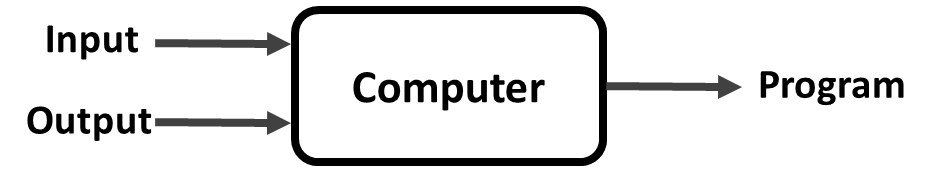
\includegraphics[width=0.7\linewidth]{supervised_learning}
			\caption{Supervised learning}
			\label{fig:supervisedlearning}
		\end{figure}
	\end{solution}
	
	\question[15]
	What are the main types of deep reinforcement learning algorithms? What is the goal of each approach?
	
	\begin{solution}
		Deep learning algorithms can be classified based on their strategy for finding the optimal policy.
		
		Value learning: The goal is learning a $Q$ value function, that can be used to find the optimal policy:
		\[
		\pi^*(s) = \argmax_{a}{Q(s,a)}
		\]
		
		Policy learning: The goal is to directly learn the optimal policy without explicitly estimating the value function. It estimates the policy using a parameterized function, which is fine tuned through a learning process.
		\[
		\pi^*(s) \sim \pi(s)
		\]
	\end{solution}
	
	\newpage
	\question[30]
	A genetic algorithm uses binary coded individuals. In a given generation, there are 6 individuals:
	\begin{align*}
		x_1 &=  \left[ 0110111001 \right], \text{fitness}: 5 \\
		x_2 &=  \left[ 0101100101 \right], \text{fitness}: 27 \\
		x_3 &=  \left[ 1010011100 \right], \text{fitness}: 30 \\
		x_4 &=  \left[ 0010010011 \right], \text{fitness}: 33 \\
		x_5 &=  \left[ 1101101100 \right], \text{fitness}: 5 \\
		x_6 &=  \left[ 1010101010 \right], \text{fitness}: 100 \\
	\end{align*}
	Using roulette wheel selection, calculate the expected number of copies of each individual in the crossover while maintaining a constant population size, i.e. select 6 parents, which will be the parents during the crossover! Illustrate the crossover with the selected parent individuals, and then also show the mutation with uniform mutation, assuming a mutation probability of $5\%$ per bit!
	\begin{solution}
		\begin{table}[H]
			\centering
			\begin{tabular}{|c|c|c||c|c|c|}
				\hline
				no. & Initial population & Fitness & $\Pr_i$ & Expected count & Actual count \\
				\hline
				1 & $0110111001$ & $5$ & $0.025$ & $0.15$ & $0$ \\
				2 & $0101100101$ & $27$ & $0.135$ & $0.81$ & $1$ \\
				3 & $1010011100$ & $30$ & $0.15$ & $0.9$ & $1$  \\
				4 & $0010010011$ & $33$ & $0.165$ & $0.99$ & $1$ \\
				5 & $1101101100$ & $5$ & $0.025$ & $0.15$  & $0$ \\
				6 & $1010101010$ & $100$ & $0.5$ & $3$ & $3$ \\
				\hline
				Sum & & $200$ & $1.0$ & $6$ & $6$ \\
				\hline
			\end{tabular}
			\caption{Selection}
		\end{table}
		
		\begin{table}[H]
			\centering
			\begin{tabular}{|c|c||c|c|}
				\hline
				no. & Mating pool & Crossover point & Offspring \\
				\hline
				2 & $01 \mid 01100101$ & $2$ & $01 \mid 10011100$ \\
				3 & $10 \mid 10011100$ & $2$ & $10 \mid 01100101$ \\
				4 & $0010 \mid 010011$ & $4$ & $0010 \mid 101010$   \\
				6 & $1010 \mid 101010$ & $4$ & $1010 \mid 010011$  \\
				6 & $101010 \mid 1010$ & $6$ & $101010 \mid 1010$  \\
				6 & $101010 \mid 1010$ & $6$ & $101010 \mid 1010$ \\
				\hline
			\end{tabular}
			\caption{Crossover}
		\end{table}
		
		We simulate a $5\%$ chance by flipping every 20th bit.
		
		\begin{table}[H]
			\centering
			\begin{tabular}{|c|c||c|}
				\hline
				no. & Offspring & Offspring after mutation \\
				\hline
				2 & $0110011100$ & $0110011100$  \\
				3 & $100110010\underline{1}$ & $100110010\underline{0}$  \\
				4 & $0010101010$ & $0010101010$    \\
				6 & $101001001\underline{1}$ & $101001001\underline{0}$   \\
				6 & $1010101010$ & $1010101010$   \\
				6 & $101010101\underline{0}$ & $101010101\underline{1}$  \\
				\hline
			\end{tabular}
			\caption{Mutation}
		\end{table}
	\end{solution}
	
	\question[15]
	What components affect the weight modification in Perceptron's training algorithm.
	
	\begin{solution}
		The learning rate and the output of the activation function.
	\end{solution}
	
	\question[15]
	In the Schelling model, what will agent A do if its tolerance level is $45\%$, its color is RED, and it is in the following neighborhood:
	\begin{table}[H]
		\centering
		\begin{tabular}{|c|c|c|}
			\hline
			RED & BLUE & RED \\ \hline
			BLUE & Agent A & BLUE \\ \hline
			RED & BLUE & RED \\ \hline
		\end{tabular}
	\end{table}
	
	\begin{solution}
		The agent will move, since $\frac{4}{8} = 50\%$ of the agent's neighbours are BLUE which is higher then their tolerance level.
	\end{solution}
\end{questions}
\newpage
\subsection{B}
\begin{questions}
	\question[10]
	What does the "Coffee Test" (designed to test artificial general intelligence) consist of?
	
	\begin{solution}
		The machine enters an average home and figures out how to brew coffee:
		\begin{itemize}
			\item finds the coffee machine
			\item finds the coffee
			\item adds water
			\item finds a mug
			\item brews the coffee by the proper use of the machine
		\end{itemize}
	\end{solution}
	
	\question[15]
	What is the unsupervised learning method? Draw a figure to introduce the mechanisms of the method!
	
	\begin{solution}
		Sometimes labelled data is unavailable and in some cases not even its classes and characteristics of are known. The solution to this problem is the group similar data together in so called clusters.
			
		Unsupervised learning takes a given set of unlabeled data, and produces output data (labels) and a function, which maps input to output.
		
		\begin{figure}[H]
			\centering
			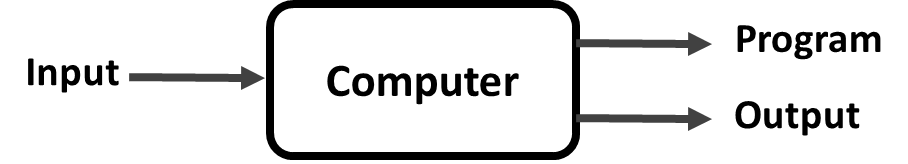
\includegraphics[width=0.7\linewidth]{unsupervised_learning}
			\caption{Unsupervised learning}
			\label{fig:unsupervisedlearning}
		\end{figure}
	\end{solution}
	
	\question[15]
	What components affect the flight vector of a particle in a PSO algorithm?
	
	\begin{solution}
		\begin{itemize}
			\item current position
			\item current velocity
			\item distance between current position and pbest
			\item distance between current position and gbest
		\end{itemize}
	\end{solution}
	
	\newpage
	\question[30]
	In a wrestling competition, wrestlers are divided into leagues based on their height and weight. Divide the competitors into two leagues ($k=2$) based on the data obtained using the k-means algorithm. Perform the calculation over two iterations, taking the values of the first and second competitors as the initial center points.
	
	\begin{table}[H]
		\centering
		\begin{tabular}{|c|c|c|}
			\hline
			ID & height (cm) & weight(kg) \\ \hline \hline
			1 & 185 & 76 \\ \hline
			2 & 170 & 66 \\ \hline
			3 & 168 & 68 \\ \hline
			4 & 179 & 74 \\ \hline
			5 & 182 & 73 \\ \hline
			6 & 188 & 75 \\ \hline
		\end{tabular}
	\end{table}

	
	\begin{solution}
		First iteration:	
		\begin{figure}[H]
			\centering
			\begin{tikzpicture}
				\begin{axis}[
					enlargelimits=0.2,
					scatter/classes={
						a={mark=square*,green},
						b={mark=square*,red},
						am={mark=circle*,red},
						bm={mark=circle*,green},
						c={blue}
					}
				]
					
				\addplot[
					scatter, mark=*, only marks, 
					scatter src=explicit symbolic,
					nodes near coords*={\Label},
					visualization depends on={value \thisrow{label} \as \Label}
				] table [meta=class] {
					x y class label
					185 76 a 1
					170 66 b 2
					168 68 c 3 
					179 74 c 4
					182 73 c 5 
					188 75 c 6
				};
				\end{axis}
			\end{tikzpicture}
			\caption{Initialize center points}
		\end{figure}
		
		\begin{figure}[H]
			\centering
			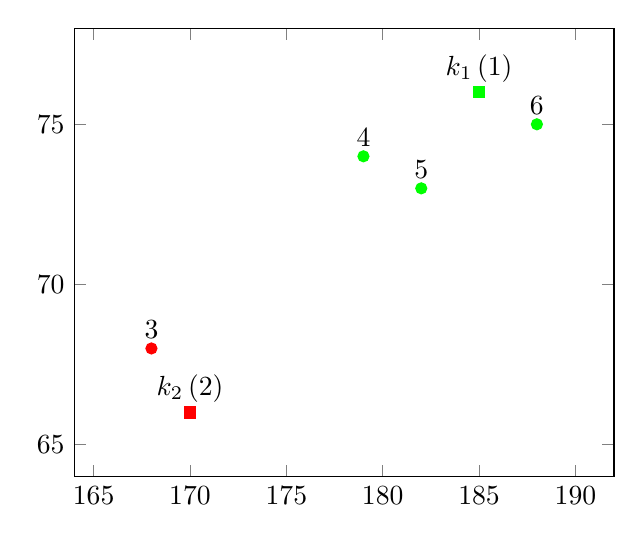
\begin{tikzpicture}
				\begin{axis}[
					enlargelimits=0.2,
					scatter/classes={
						a={mark=square*,green},
						b={mark=square*,red},
						am={red},
						bm={green},
						c={blue}
					}
					]
					
					\addplot[
					scatter, mark=*, only marks, 
					scatter src=explicit symbolic,
					nodes near coords*={\Label},
					visualization depends on={value \thisrow{label} \as \Label}
					] table [meta=class] {
						x y class label
						185 76 a $k_1\,(1)$ 
						170 66 b $k_2\,(2)$ 
						168 68 am 3 
						179 74 bm 4
						182 73 bm 5 
						188 75 bm 6
					};
				\end{axis}
			\end{tikzpicture}
			

			\caption{Assign points to nearest center}
		\end{figure}
		Recalculate cluster centers:
		\begin{align*}
			k_1 &= \left(\frac{185 + 179 + 182 + 188}{4}, \frac{76 + 74 + 73 + 75}{4} \right) = \left(183.5, 74.5 \right) \\
			k_2 &= \left(\frac{170 + 168}{2}, \frac{66 + 68}{2} \right) = \left(169, 67 \right) 
		\end{align*}
		
		\begin{figure}[H]
			\centering
			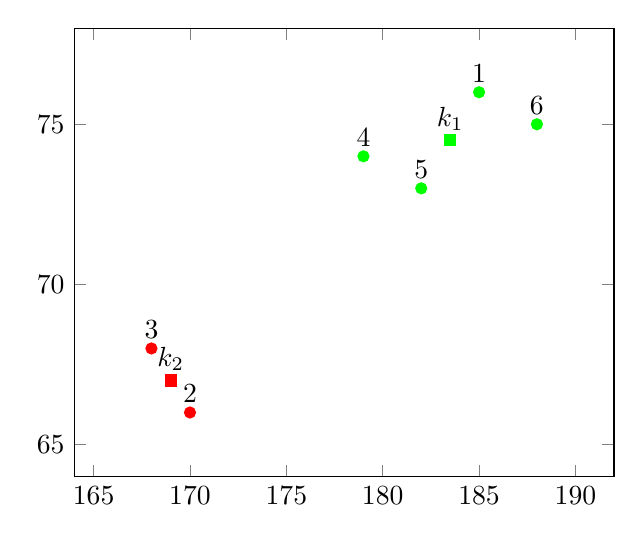
\begin{tikzpicture}
				\begin{axis}[
					enlargelimits=0.2,
					scatter/classes={
						a={mark=square*,green},
						b={mark=square*,red},
						am={red},
						bm={green},
						c={blue}
					}
					]
					
					\addplot[
					scatter, mark=*, only marks, 
					scatter src=explicit symbolic,
					nodes near coords*={\Label},
					visualization depends on={value \thisrow{label} \as \Label}
					] table [meta=class] {
						x y class label
						183.5 74.5 a $k_1$
						169 67 b $k_2$
						185 76 bm 1
						170 66 am 2
						168 68 am 3 
						179 74 bm 4
						182 73 bm 5 
						188 75 bm 6
					};
				\end{axis}
			\end{tikzpicture}
			
			\caption{Move cluster centers}
		\end{figure}
		Second iteration: Based on the new center points, the points need to be reassigned. In our case no points change ownership resulting in the termination of the algorithm.
	\end{solution}
	

	

	
	\question[15]
	What are the downsides of using a Q-learning method?
	
	\begin{solution}
		\begin{itemize}
			\item only works on discrete action spaces
			\item policy is computed deterministically, so the model cannot learn stochastic policies 
		\end{itemize}
	\end{solution}
	
	\question[15]
	In the Schelling model, what will agent A, do if its tolerance level is $55\%$, its color is RED and it is in the following neighborhood:
	
	\begin{table}[H]
		\centering
		\begin{tabular}{|c|c|c|}
			\hline
			RED & BLUE & RED \\ \hline
			BLUE & Agent A & BLUE \\ \hline
			RED & BLUE & RED \\ \hline
		\end{tabular}
	\end{table}
	
	\begin{solution}
		The agent will not move, since $\frac{4}{8} = 50\%$ of the agent's neighbours are BLUE which is lower then their tolerance level.
	\end{solution}
\end{questions}

\end{document}
